%!TEX program = xelatex
\documentclass[12pt]{article}

\usepackage[english]{babel}
\usepackage{xeCJK}

% Set page size and margins
\usepackage[a4paper,top=2cm,bottom=2cm,left=3cm,right=3cm,marginparwidth=1.75cm]{geometry}

% Useful packages
\usepackage{amsmath}
\usepackage{graphicx}
\usepackage[colorlinks=true, allcolors=blue]{hyperref}

\usepackage{array}
\newcolumntype{P}[1]{>{\centering\arraybackslash}p{#1}}
\newcolumntype{M}[1]{>{\centering\arraybackslash}m{#1}}

\usepackage{adjustbox}
\usepackage{caption}
\usepackage{subcaption}
\usepackage{siunitx}
\usepackage{float}
\usepackage{subfloat}

% ----- paragraph -----
\usepackage{titlesec}
\setcounter{secnumdepth}{4}
\titleformat{\paragraph}
{\normalfont\normalsize\bfseries}{\theparagraph}{1em}{}
\titlespacing*{\paragraph}
{0pt}{3.25ex plus 1ex minus .2ex}{1.5ex plus .2ex}
% ----- paragraph ----

\setCJKmainfont{NotoSerifTC-Regular}[
  AutoFakeBold = 3
]

\usepackage{indentfirst}
\setlength\parindent{24pt}

\begin{document}

\begin{titlepage}
  \begin{center}
      \vspace*{1cm}
       \begin{LARGE} 
           \textbf{
           \\ 數位電路實驗結報一
           \\ \
           \\ --6-bit 數位加法器--
           }
       \end{LARGE}
      \vspace{0.5cm}
        \textbf{}
          
      \vspace{1.5cm}

      \textbf{Group 2: B11303052 蘇盈翰 (Right), B11702091 張容爾 (Middle), B10901144 王俊皓 (Left)}
       
      \vspace{1.5cm}

      \text{\today}

      \vspace{0.8cm}

      
\includegraphics[width=0.7\textwidth]{figure/Member.jpg}
     
      \vfill
          
      \vspace{0.8cm}
     
  \end{center}
\end{titlepage}

\section{實驗原理}

\subsection{半加器與全加器 (Half Adder \& Full Adder)}
加法器為數位邏輯電路中執行二進位加法運算之核心元件。最基本的\textbf{半加器}負責兩個單一位元 $\mathrm{A}$ 與 $\mathrm{B}$的加法，其輸出包含總和 ($\mathrm{S}$) 與進位 ($\mathrm{C_{out}}$)，布林邏輯表示式為：
\begin{gather}
   \mathrm{S} = \mathrm{A} \oplus \mathrm{B} \\
   \mathrm{C_{out}} = \mathrm{A} \cdot \mathrm{B}
\end{gather}

為了處理多位元的加法，必須考慮來自較低位元的進位。因此引入了\textbf{全加器}，它包含三個輸入端：兩個加數 ($\mathrm{A}$, $\mathrm{B}$) 以及一個進位輸入 ($\mathrm{C_{in}}$)。全加器的輸出邏輯表示式為：
\begin{gather}
   \mathrm{S} = \mathrm{A} \oplus \mathrm{B} \oplus \mathrm{C_{in}} \\
   \mathrm{C_{out}} = (\mathrm{A} \cdot \mathrm{B}) + (\mathrm{C_{in}} \cdot (\mathrm{A} \oplus \mathrm{B}))
\end{gather}

\subsection{邏輯閘實現與笛摩根定理}
在實際的電路中，我們使用 IC 7486 (XOR 閘) 與 IC 7400 (NAND 閘) 來建構上述邏輯。

對於總和 $\mathrm{S}$ 可以直接透過兩個 XOR 閘串接完成，而進位 $\mathrm{C_{out}}$ 的部分，原本的設計需要 AND 閘與 OR 閘，為了僅使用 NAND 閘 (IC 7400) 來完成進位電路，我們可套用\textbf{笛摩根定理 (De Morgan's Laws)} 將原本的 AND-OR 形式轉換為 NAND-NAND 形式：
\begin{equation}
   \mathrm{C_{out} = \overline{ \overline{(A \cdot B)} \cdot \overline{(C_{in} \cdot (A \oplus B))} }}
\end{equation}
透過此轉換，即可大幅簡化所需的 IC 種類，完全依靠 IC 7486（XOR 閘）與 IC 7400 (NAND 閘) 實現 1-bit 全加器。

\subsection{漣波進位加法器 (Ripple Carry Adder)}
要實現多位元（如本實驗之 6-bit）的加法運算，可將多個全加器串聯組成「漣波進位加法器」。其原理是將第 $\mathrm{i}$ 個位元的進位輸出 ($\mathrm{C_{out, i}}$) 直接連接至第 $i+1$ 個位元的進位輸入 ($\mathrm{C_{in, i+1}}$)。

本次實驗中，我們將兩個現成的 3-bit 加法器模組進行擴充，把低位元 (Lower 3-bits) 加法器的最高位進位輸出，連接至高位元 (Upper 3-bits) 加法器的最低位進位輸入 ($\mathrm{C_{in}}$)，藉由進位訊號的傳遞 (Carry Propagation)，成功構建出完整的 6-bit 數位加法器。

\section{實驗架設與步驟}

\subsection{1-bit 數位加法器實作 (實驗一)}
\begin{enumerate}
   \item \textbf{硬體接線：}
   \begin{itemize}
       \item 準備 IC 7486 與 IC 7400，將其固定於麵包板上。分別將兩顆 IC 的第 14 腳位連接至 ADALM2000 提供的 +5V 電源 (VCC)，第 7 腳位連接至接地 (GND)。
       \item 依據理論化簡後之電路圖進行佈線：利用 7486 負責處理總和 ($\mathrm{S}$) 與部分進位邏輯，並將其輸出結果接入 7400 進行 NAND 邏輯運算，以產生最終的進位輸出 ($\mathrm{C_{out}}$)。
       \item 將 ADALM2000 的數位腳位 (DIO) 連接至電路對應節點：DIO 0 接至輸入 $\mathrm{A}$、DIO 1 接至輸入 $\mathrm{B}$、DIO 2 接至輸入 $\mathrm{C_{in}}$；量測端的部分，將 DIO 3 接至總和輸出  $\mathrm{S}$、DIO 4 接至進位輸出 $\mathrm{C_{out}}$。
   \end{itemize}
   \begin{center}
       \begin{figure}[H]
           \centering
           \includegraphics[width=0.4\textwidth]{figure/IC 1 bit layout.png}
           \caption{1-bit 全加器電路實作圖}\label{fig:waveform_1bit}
       \end{figure}
   \end{center}
   \item \textbf{軟體設定 (Scopy)：}
   \begin{itemize}
       \item \textbf{Pattern Generator (訊號產生器)：} 開啟 Scopy 軟體，將 DIO 0、1、2 設定為 Binary Counter 模式，並設定為三個等比頻率（例如 $\mathrm{A}$ 設為 4 kHz、$\mathrm{B}$ 設為 2 kHz、$\mathrm{C_{in}}$ 設為 1 kHz）。此設定可產生所有 8 種 0 與 1 的輸入排列組合。
       \item \textbf{Logic Analyzer (邏輯分析儀)：} 開啟 DIO 0 至 DIO 4 的波形顯示。將取樣率 (Sample Rate) 設定為 5 Msps，取樣數量 (Nr of samples) 設定為 20k Samples。
       \item 擷取波形，觀察輸出腳位與輸入腳位之電位變化，並比對全加器真值表以驗證硬體邏輯。
   \end{itemize}
\end{enumerate}

\subsection{多位元加法器串聯測試 (實驗二)}
\begin{itemize}
   \item \textbf{3-bit 加法器模組測試：} 取得助教事先製作的 3-bit 加法器電路板，透過板上的指撥開關給定不同的輸入組合，並觀察 LED 燈亮的狀態來驗證 3-bit 的加法結果（例如測試 $3+5=8$，即二進位之 $011_2 + 101_2 = 1000_2$）。
       \begin{figure}[H]
           \centering
           \includegraphics[width=0.4\textwidth]{figure/IC 3 bits layout.png}
           \caption{3-bit 全加器電路實作圖}\label{fig:waveform_3bit}
       \end{figure}
   \item \textbf{6-bit 加法器擴充：} 將兩塊 3-bit 加法器模組進行串聯。把處理低位元 (Lower 3-bits) 模組的進位輸出端 ($\mathrm{C_{out}}$)，利用跳線連接至處理高位元 (Upper 3-bits) 模組的進位輸入端 ($\mathrm{C_{in}}$)。
       \begin{figure}[H]
           \centering
           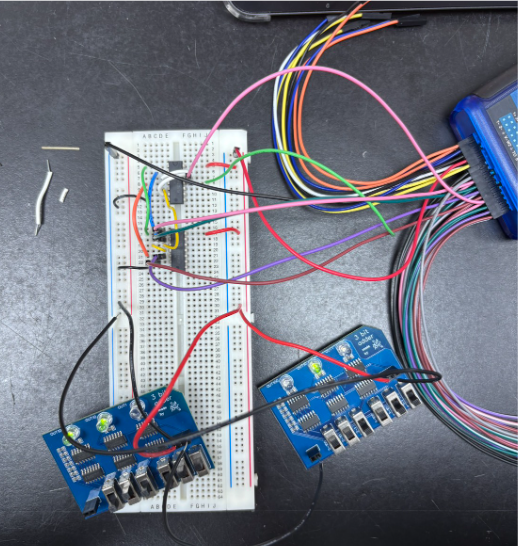
\includegraphics[width=0.4\textwidth]{figure/IC 6 bits layout.png}
           \caption{6-bit 全加器電路實作圖}\label{fig:waveform_6bit}
       \end{figure}
   \item 透過 ADALM 再次進行輸入測試，確認進位訊號能順利跨模組傳遞，完成並驗證完整的 6-bit 加法運算邏輯。
\end{itemize}

\section{實驗結果與分析}

\subsection{1-bit 數位全加器邏輯驗證}
透過 ADALM2000 擷取訊號，我們記錄了 1-bit 全加器在 8 種不同輸入組合下的輸出結果（如表 \ref{table:truth_table} 所示）。分析該測量數據可得出以下結論：
   \begin{center}
       \begin{table}[H]
       \centering
       \renewcommand{\arraystretch}{1.2} % 增加行高，讓表格看起來不那麼擁擠
       \begin{tabular}{|c||c|c|c|c|c|c|c|c|}
       \hline
       \textbf{狀態} & \textbf{1st} & \textbf{2nd} & \textbf{3rd} & \textbf{4th} & \textbf{5th} & \textbf{6th} & \textbf{7th} & \textbf{8th} \\ \hline \hline
       \textbf{A}    & 1 & 0 & 1 & 0 & 1 & 0 & 1 & 0 \\ \hline
       \textbf{B}    & 0 & 1 & 1 & 0 & 0 & 1 & 1 & 0 \\ \hline
       \textbf{$\mathrm{C_{in}}$}  & 0 & 0 & 0 & 1 & 1 & 1 & 1 & 0 \\ \hline
       \textbf{S}    & 1 & 1 & 0 & 1 & 0 & 0 & 1 & 0 \\ \hline
       \textbf{$\mathrm{C_{out}}$} & 0 & 0 & 1 & 0 & 1 & 1 & 1 & 0 \\ \hline
       \end{tabular}
       \caption{1-bit 全加器輸入與輸出之實測真值表}
       \label{table:truth_table}
       \end{table}
   \end{center}
\begin{itemize}
   \item \textbf{總和 ($\mathrm{S}$) 邏輯分析：} 當輸入端 $\mathrm{A, B, C_{in}}$ 中有「奇數」個 1 處於高電位時（即狀態 1st, 2nd, 4th, 7th），總和輸出 $\mathrm{S}$ 皆為 1。這完美吻合 XOR 閘 ($\mathrm{A \oplus B \oplus C_{in}}$) 的奇偶校驗 (Parity Check) 特性。
   \item \textbf{進位 ($\mathrm{C_{out}}$) 邏輯分析：} 當輸入端有「兩個或三個」 1 處於高電位時（即狀態 3rd, 5th, 6th, 7th），進位輸出 $\mathrm{C_{out}}$ 皆為 1。這證明了我們利用 IC 7400 (NAND 閘) 配合笛摩根定理所建構的進位電路，成功實現了全加器的多數決邏輯 (Majority Logic)。
\end{itemize}
實測之數位波形電壓與理論真值表完全吻合，證實本實驗的硬體佈線與邏輯化簡皆正確無誤。
\begin{figure}[H]
   \centering
   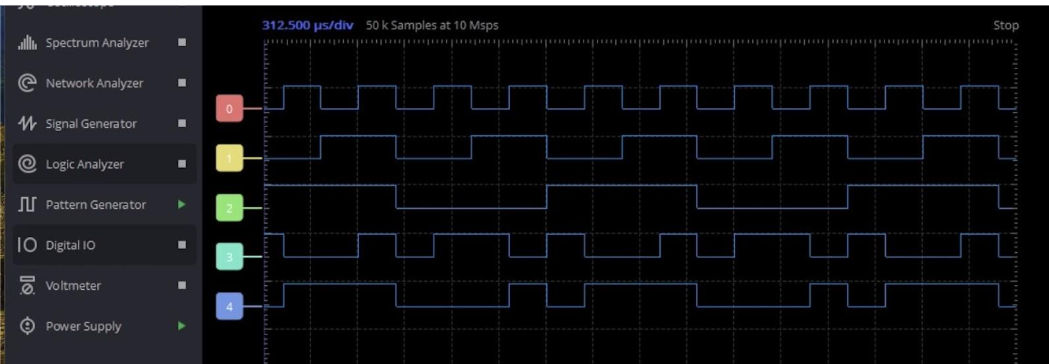
\includegraphics[width=0.7\textwidth]{figure/output wave front.png}
   \caption{1-bit 全加器輸入與輸出之實測波形圖}\label{fig:waveform}
\end{figure}

\subsection{6-bit 加法器串聯結果與訊號傳遞分析}
在進階實驗中，我們成功將兩個 3-bit 加法器模組串接，擴充為完整的 6-bit 加法器。測試過程中，我們輸入了多組十進位加法進行二進位驗證。例如測試 $3 + 5 = 8$ 時（即二進位之 $000011_2 + 000101_2$）：

運算過程觀察：由於低位元（第1、2個 bit）的相加產生了進位，我們可以觀察到低位元模組的 $\mathrm{C_{out}}$ 輸出高電位，並成功觸發高位元模組的 $\mathrm{C_{in}}$ 接收端，最終正確點亮對應 $1000_2$ （即數值 8）的輸出 LED 燈。


然而，此種架構存在一個固有的效能瓶頸：每一個位元的進位輸出必須等待前一級的進位計算完成後才能進行，導致時間的延遲隨位元數增加而線性累積。為了改善此問題，可引入超前進位加法器（Carry Lookahead Adder, CLA），其概念是透過額外的硬體邏輯，提前計算出各個位元是否會產生或傳遞進位，從而打破逐級等待的限制，大幅提升數位電路的運算效能。

\section{問題討論}


\subsection{為什麼 LED 矩陣的腳位會這麼亂，有什麼好處嗎？}
站在設計者角度的話，會根據配合驅動IC的腳位，進而去設定8*8的LED陣列腳位，就好像dynamic duo一樣，產品一套賣出，對買者有良好的使用一致性體驗，賣家和設計者也能藉此商機多賺一筆。而LED陣列有一個最主要的配合驅動IC，就是MAX7219。要問LED陣列為什麼這麼亂，就得追本溯源，問MAX7219的腳位為何？
查詢後，果然MAX7219 腳位看起來亂，是因為它不是照「數字順序」排，而是照「電流、晶片內部 layout、封裝腳位、七段顯示器/LED matrix 走線」排。
而你若細看MAX7219，他有DIG和SEG兩種port，DIG選擇8個column中哪些要亮，SEG選擇每個colunm中，哪幾顆LED要亮。
了解此，進而去細究DIG的腳位配置，觀察sequence{04623751}的規律，這是個Gray code like sequence，若要用Gray code去理解IC腳位設計的話，Gray code cube使得腳位間的電訊號更好地利用SIPO這特點。這使得。而Gray code有一個最主要的encode特徵，相鄰兩點只差一個bit variance。舉例來說，在Gray code Cube上，{000}的鄰居有，{001},{010},{100}，也就是說腳位1的鄰居是腳位1,2,4。這種設計，優化了decoder/driver layout設計。
接下來要了解的SEG腳位設計，這種設計是為了迎合七段顯示器的的掃描順序，AFBGCED，這樣的腳位安排能將此IC更好地融合到七段顯示器上。


\subsection{電視或電腦等更多像素的螢幕是怎麼控制的，與今天電路的相似與相異之處？}
電視或電腦螢幕雖然像素數量比今天的 LED 矩陣多非常多，但基本概念其實相似：它們都是把畫面切成一個二維矩陣，用「列」和「行」的方式來控制每個像素的位置。今天的 LED 矩陣是利用 row 和 column 交會的位置來點亮 LED，例如先選擇某一列，再決定這一列中的哪些欄要亮；電視和電腦螢幕也是依照類似的掃描概念，一列一列地更新畫面。
以電腦螢幕為例，GPU 會先在記憶體中產生一張完整的畫面，這張畫面叫做 framebuffer，裡面記錄了每個像素的顏色資訊，例如紅、綠、藍三個數值。接著，GPU 會透過 HDMI、DisplayPort 或筆電內部的 eDP，把這些影像資料高速傳送到螢幕。螢幕內部的 timing controller，簡稱 TCON，會接收這些資料，並控制面板內部的 row driver 和 column driver，把資料送到正確的位置。
如果是 LCD 螢幕，每個像素本身不會發光，而是透過液晶控制背光能不能通過。LCD 面板中每個像素旁邊都有一個很小的 TFT 電晶體，可以把它想成一個微小開關。螢幕會先選擇某一列，打開那一列所有像素的 TFT，然後 column driver 把每個像素需要的電壓送進去。這個電壓會暫存在像素旁邊的小電容中，讓液晶在下一次更新前維持同樣的透光程度。也就是說，LCD 的掃描不是「掃到才亮」，而是「掃到時寫入資料，之後像素自己保持狀態」。
如果是 OLED 或 AMOLED 螢幕，每個像素本身會發光，所以它更像是超大型、超精密的 LED 矩陣。不過它也不是用簡單的被動掃描方式，因為螢幕像素太多，如果每一列只在掃描到時才亮，亮度會太低、瞬間電流會太大。因此 OLED 螢幕通常也使用 active matrix 結構，每個像素附近都有 TFT 和儲存電容，用來記住亮度資料，並在一整個 frame 期間持續控制 OLED 發光。
這和今天的 LED 矩陣電路有幾個相似處。第一，它們都是矩陣結構，都可以用 row 和 column 來定位像素。第二，它們都使用掃描概念，不是每個像素都獨立拉一條控制線，而是透過一列一列或一行一行的方式更新畫面。第三，它們都需要 driver IC 幫忙控制大量輸出腳位，像今天用 MAX7219 控制 8×8 LED 矩陣，而大螢幕則使用更複雜的 TCON、source driver 和 gate driver。
但兩者也有很大的不同。今天的 LED 矩陣比較接近被動矩陣控制，LED 通常只有亮或不亮，控制方式比較單純；而電視和電腦螢幕的像素數量可能有幾百萬甚至上千萬個，每個像素還要
顯示不同亮度與顏色，所以需要更複雜的灰階控制、電壓控制或電流控制。LED 矩陣通常是掃到某一列時才讓那一列發光，而現代 LCD、OLED 螢幕多半是主動矩陣，掃描時只是把資料寫進像素，之後像素會靠 TFT 和電容維持狀態。
因此，可以說今天的 LED 矩陣是現代螢幕控制原理的簡化模型。兩者共同的核心都是「矩陣、掃描、driver IC、row/column 控制」；不同的是，電視和電腦螢幕因為像素數量巨大、需要彩色與灰階顯示，所以加入了 GPU、framebuffer、高速影像傳輸、TCON、TFT、儲存電容和類比驅動電路。簡單來說，今天的電路是在直接掃描點亮 LED；現代螢幕則是先由 GPU 產生畫面資料，再由螢幕內部電路把資料逐列寫入每個像素，讓整個畫面穩定顯示出來。


\end{document}